\section{Benchmarking the~AWBS nonlocal transport model}
\label{sec:BenchmarkingAWBS}
After having shown several encouraging properties of the~AWBS transport 
equation defined by \eqref{eq:AWBS_model} under local diffusive conditions
in \secref{sec:DiffusiveKinetics}, this section focuses on analyzing 
its behavior under nonlocal plasma conditions, extensively investigated 
in numerous publications 
\cite{Malone_1975_15, Colombant_PoP2005, Bell_1981_83, LMV_1983_7, Brantov_Nonlocal_electron_transport_1998, schurtz2000, Sorbo_2015}.
A~variety of tests suitable for benchmarking the~nonlocal electron 
transport models have been published 
\cite{Epperlein_PoFB1991, marocchino2013, Sorbo_2015, 
Sorbo_2016, Sherlock_PoP2017, Brodrick_PoP2017}, we focus on 
conditions relevant to inertial confinement fusion plasmas generated by lasers.

We show results of our implementation of the~AP1 nonlocal transport model 
presented in \secref{sec:AWBSnonlocal} benchmarked against simulation results 
provided by a~rather complete set of kinetic models with varying complexity. 
The~most reliable model represents Calder, a~collisional Particle-In-Cell
code resolving the~plasma frequency time scale, then a~standard VFP model
represented by Aladin and Impact \cite{Kingham_JCP2004}, 
and last but not least we adopt the~simplest kinetic approach represented by
SNB nonlocal model \cite{Schurtz_2000} used on the~hydrodynamic time scale. 
It should be stressed that it is a~first time when a~collisional PIC is used
in benchmarking of nonlocal electron transport models. 
%Their description follows in the~next section.

%\begin{figure}[tbh]
%  \begin{center}
%    \begin{tabular}{c}
%      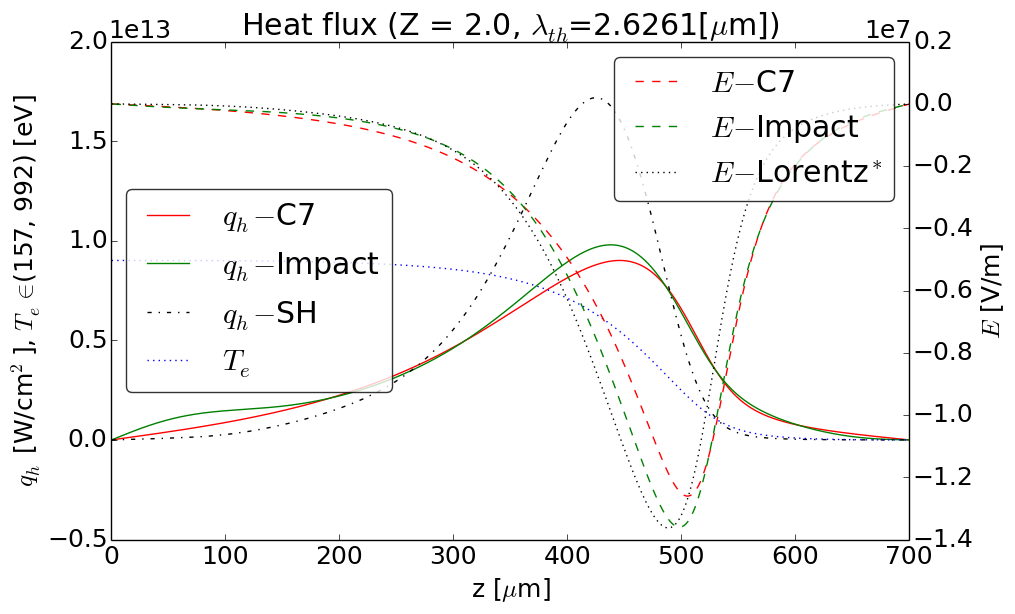
\includegraphics[width=\figscale\textwidth]{../VFPdata/C7_Impact_case3_heatflux.png} \\
%      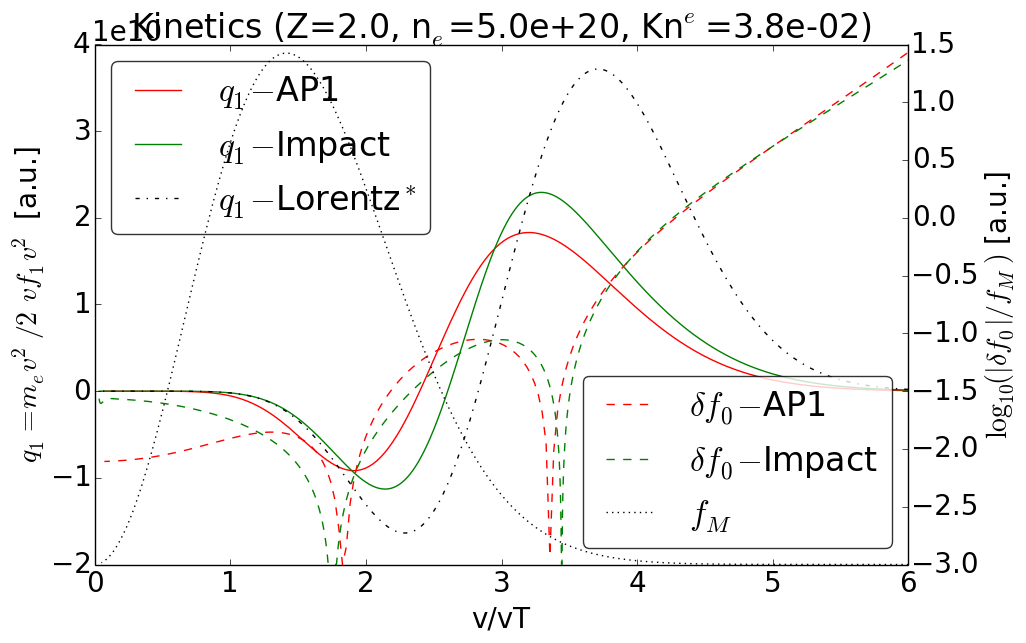
\includegraphics[width=\figscale\textwidth]{../VFPdata/C7_Impact_case3_kinetics.png}
%    \end{tabular}
%  \caption{  
%  Snapshot 12 ps. Left: correct steady solution of heat flux. 
%  Right: correct comparison to kinetic profiles at point 437 $\mu$m by Impact.
%  Velocity limit 4.0 $\vth$.
%  }
%  \label{fig:C7_Impact_case3}
%  \end{center} 
%\end{figure}

%\subsection{Aladin, Impact, and Calder kinetic codes}
%\label{sec:AladinImpactCaldercodes}

%%% CEA contribution starts
\textbf{Calder PIC code}

A~fluid description of the~particle 
phase-space, including small angle binary collisions, can be described with 
the~Maxwell equations \eqref{eq:Faraday}, \eqref{eq:Ampere}
%\begin{eqnarray}
%&&\nabla\cdot \mathbf{E}=\sum_\alpha \frac{q_\alpha}{\varepsilon_0} n_{\alpha},\\
%&&\nabla\cdot \mathbf{B}=0,\\
%&&\nabla\vect{\times} \mathbf{E}+\frac{\partial \mathbf{B}}{\partial t}=0,\\
%&&\nabla\vect{\times} \mathbf{B}-\mu_0\varepsilon_0\frac{\partial \mathbf{E}}{\partial t}=\mu_0\sum_\alpha\mathbf{j}_{\alpha},\label{maxw}
%\end{eqnarray}
coupled with the~ion and electron Vlasov equations with 
the~Landau-Beliaev-Budker collisions integral (LBB)
\cite{Landau_1936, Beliaev_SPD1956} 
\begin{multline}
\frac{\partial f_\alpha}{\partial t}+\mathbf{v}\cdot\nabla_{\mathbf{x}}f_\alpha+q_\alpha\left(\mathbf{E}+\mathbf{v}\vect{\times}\mathbf{B}\right)\nabla_{\mathbf{p}}f_\alpha =
\\
C_{LBB}(f_\alpha,f_\alpha)+\sum_\beta C_{LBB}(f_\alpha,f_\beta)
.
\end{multline}
The LBB collision integral takes the~form
\begin{multline}
C_{LBB}(f_\alpha,f_\beta)=
\\
-\frac{\partial}{\partial \mathbf{p}}\cdot\frac{\Gamma_{\alpha\beta}}{2}\left[\int \mathbf{U}(\mathbf{p},\mathbf{p}^\prime)\cdot(f_\alpha\nabla_{\mathbf{p}^\prime}f_\beta^\prime-f_\beta^\prime\nabla_{\mathbf{p}}f_\alpha)\right]d^3\mathbf{p}^\prime
,
\label{eq:LBB_model}
\end{multline}
where its relativistic kernel reads
$\mathbf{U}(\mathbf{p},\mathbf{p}^\prime)=\frac{r^2/\gamma\gamma^\prime}{(r^2-1)^{3/2}}$ 
$\left[(r^2-1)\mathbf{I}-\mathbf{p}\otimes\mathbf{p}-\mathbf{p}^\prime\otimes\mathbf{p}^\prime+r(\mathbf{p}\otimes\mathbf{p}^\prime+\mathbf{p}^\prime\otimes\mathbf{p})\right]$
with $\gamma=\sqrt{1+\mathbf{p}^2}$, $\gamma^\prime=\sqrt{1+\mathbf{p}^{\prime 2}}$ and $r=\gamma\gamma^\prime-\mathbf{p}\cdot\mathbf{p}^\prime$. 
The momemtum $\mathbf{p}_\alpha$ ($\mathbf{p}_\beta$) is normalized to 
$m_\alpha c$ (resp. $m_\beta c$). The~collision operator \eqref{eq:LBB_model} 
tends to \eqref{eq:LFP_model} in the non-relativistic limit.
%described in Appendix~\ref{app:CalderKinetics}. 
%The~latter is the~relativistic version of the~collision operator 
%introduced in \eqref{eq:LFP_model}. 
The aforementioned model is solved in 3D by the PIC code CALDER. 
\cite{Lefebvre_NF2003, Perez_PoP2012}.

Brief description of the Calder code \figref{fig:C7_Calder_case1}.

\textbf{Impact and Aladin VFP codes}

The~PIC code is extremely expensive as the~collisions require the~description 
of the~velocity space in 3 dimensions. Yet, a~reduction of dimensions can be 
done by developing the~distribution function in a~cartesian tensor series, 
equivalent to a~serie along the spherical harmonics \cite{Johnston_PR1960}.
%as follows:\textit{CPR comment - Cartesian tensors are the same as spherical harmonics to first order}
%\begin{equation}
%  f(t,\mathbf{x},\vv) = f_0(t,\mathbf{x},\vmag) 
%  + \vn\cdot \vect{f}_1(t,\mathbf{x},\vmag)
%  +\vn\otimes\vn:\matr{f}_2(t,\mathbf{x},\vmag)+... .
%  \label{Pn}
%\end{equation}
%where $v=|\mathbf{v}|$, $\Omega=\mathbf{v}/v$. 
%A P$_n$ model refers to 
%neglecting orders higher than $\matr{f}_n$. 
This in its first order form corresponds to the~P1 approximation 
\eqref{eq:P1approximation} and coupled with
%distribution function 
%approximation $f(t,\mathbf{x},\vv)\approx f_0(t,\mathbf{x},\vmag)
%+\vn\cdot \vect{f}_1(t,\mathbf{x},\vmag)$ coupled with 
the~Landau-Fokker-Planck collisional operator 
\eqref{eq:LFP_model} leads to the P$_1$-VFP model 
\cite{Johnston_PR1960, Kingham_JCP2004}:
\begin{eqnarray}
\frac{\partial \fzero}{\partial t}+\frac{\vmag}{3}\nabla \cdot \fone
+\frac{\qe}{3\me\vmag^2}\frac{\partial}{\partial \vmag}(\vmag^2\E\cdot \fone)
&=&
C^0_{ee}(\fzero) ,
 \label{eq:P1f0_Aladin}\\
\frac{\partial \fone}{\partial t}+\vmag\nabla \fzero
+ \frac{\qe\E}{\me}\frac{\partial \fzero}{\partial \vmag}
+\frac{\qe\B}{\me}\vect{\times} \fone 
&=&
- \nuei\fone .
\label{eq:P1f1_Aladin}
\end{eqnarray}
where for simplicity only a~contribution of the~isotropic part of 
the~distribution function in \eqref{eq:LFP_model} is used 
\begin{eqnarray} 
C^0_{ee}(\fzero) &=& \frac{\Gamma}{v^2}\frac{\partial}{\partial \vmag}
\left[C(f_0)f_0+D(\fzero)\frac{\partial \fzero}{\partial \vmag}\right] ,
\\
C(\fzero(\vmag)) &=& 4\pi\int_0^\vmag \fzero(u) u^2 \dI u ,
\\
D(\fzero\vmag)) &=& \frac{4\pi}{\vmag}\int_0^\vmag u^2\int_u^\infty w \fzero(w) 
\dI w \dI u .
\end{eqnarray}

Impact and Aladin solve the system \eqref{eq:P1f0_Aladin} 
and \eqref{eq:P1f1_Aladin} with the Maxwell equations  
\eqref{eq:Faraday} and \eqref{eq:Ampere} in two dimensions, 
assuming motionless ions.

It is worth mentioning that AP1 uses similar model equations as Aladin
and Impact with the~difference, that AP1 describes the~electron distribution 
function as quasi steady with respect to the~time evolution of ion fluid,
and of course, AP1 is using a~simple (linear) collision operator inherently
coupled to ion fluid via $\fM$.

Brief description of the Aladin code \figref{fig:C7_Aladin_case5}, \figref{fig:C7_Aladin_case3}.

%%% CEA contribution ends

\textbf{SNB approach}

Now considered as a~standard among nonlocal electron models in hydrodynamic 
codes, SNB \cite{Schurtz_2000} represents an efficient P1 method based on
the~velocity dependent form of the~collision BGK operator. It uses EDF 
approximation representing deviation from the~local BGK theory
\begin{equation}
  \tilde{\ft} = 
  \fM + \delta\fzero 
  + \vn\cdot\left(\fone_M + \delta\fone\right) , 
  \label{eq:SNB_approximation}
\end{equation}
where $\fone_M = - \xi\mfpei\left( \frac{\vmag^2}{2 \vth^2} - 4\right)\fM
\frac{\nabla \Te}{\Te}$ is obtained from the~diffusive solution 
\eqref{eq:BGK_approximation} with \eqref{eq:BGK_scaling}.
The~zero and first angular moment of electron transport equation 
with scaled \eqref{eq:BGK_scaling} collision operator \eqref{eq:BGK_model_1D} 
acts on SNB approximation \eqref{eq:SNB_approximation} 
as (similar to \eqref{eq:AP1f0} and \eqref{eq:AP1f1})
\begin{eqnarray}
  \frac{r \nue}{\xi}\delta\fzero &=&
  - \frac{\vmag}{3}\nabla\cdot\left(\delta\fone + \fone_M\right)
  \nonumber\\ 
  &&\xcancel{- \frac{\qe}{\me}\frac{\E}{3}\cdot\left(
  \pdv{\fone_M}{\vmag} + \pdv{\delta\fone}{\vmag} 
  + \frac{2}{\vmag}\left(\fone_M + \delta\fone\right)\right)} , 
  \nonumber \\
  \label{eq:SNBf0}\\
  \frac{\nuei}{\xi}\delta\fone &=& - \vmag\nabla\delta\fzero 
  ~\xcancel{- \frac{\qe}{\me}\E\pdv{\delta\fzero}{\vmag}} 
  \nonumber \\
  &&\underbrace{- \frac{\nuei}{\xi}\fone_M - \vmag\nabla\fM
  - \frac{\qe}{\me}\E\pdv{\fM}{\vmag}}_{~~~~~~~~~~~~~=~0,~\text{if}~\E = \E_L} 
  %+\frac{\qe\B}{\me c}\vect{\times} \left(\fone_M + \delta\fone\right)
  ,
  \nonumber \\
  \label{eq:SNBf1}
\end{eqnarray}
where the~magnetic field has been omitted. One should notice, that the~local
EDF contribution cancels out in \eqref{eq:SNBf1} when the~electric field 
adjusts to the~local Lorentz electric field \eqref{app_eq:BGK_Efield}. 
The~efficiency of SNB resides in omitting the~directional electric field 
effect (crossed out terms in \eqref{eq:SNBf0} and \eqref{eq:SNBf1}), which
leads to a~simple diffusion model 
\begin{equation}
  \frac{1}{\mfpe^{SNB}}\delta\fzero 
  - \nabla\cdot\frac{\mfpei^{SNB}}{3}\nabla\delta\fzero =
  \nabla\cdot\frac{\xi\mfpei}{3}\frac{\fM}{\Te}\nabla \Te
  ,
  \label{eq:SNB_model}
\end{equation}
where $\frac{1}{\mfpei^{SNB}} = 
\frac{\nuei}{\xi\vmag} + \frac{|\qe\E|}{\frac{1}{2}\me\vmag^2}$ 
and $\mfpe^{SNB} = \frac{\xi\vmag}{r \nue}$, and the~source term based on 
$\fone_M$ simplifies by avoiding the~bracket in the~latter. The~missing
directional effect of $\E$ in \eqref{eq:SNB_model} is mimicked as 
an~isotropic scattering in defintion of $\mfpei^{SNB}$ \cite{Schurtz_2000}.
Consequently, the~real directional effect of the~electric field in SNB
is reflected only via $\fone_M$ defined on the~basis of $\E_L$.
In this paper we porpose to use $r = \frac{1}{2}$ in accordance with 
\eqref{eq:qAWBS_approximation}. This choice gives 
$\mfpe^{SNB} = \frac{\vmag}{2.097\nue}$ in the~case of $\Zbar = 1$, 
which is in a~very good accordance with $\mfpe^{SNB} = \frac{\vmag}{2\nue}$ 
proposed in \cite{Brodrick_PoP2017}. The~explicit form of the~anistropic part of EDF then takes the~form $\fone = \fone_M - \mfpei^{SNB}\nabla\delta\fzero$.
%\begin{itemize}
%  \item Brief description of the Impact code \figref{fig:C7_Impact_case3}.
%\end{itemize}

\begin{figure}[tbh]
  \begin{center}
    \begin{tabular}{c}
      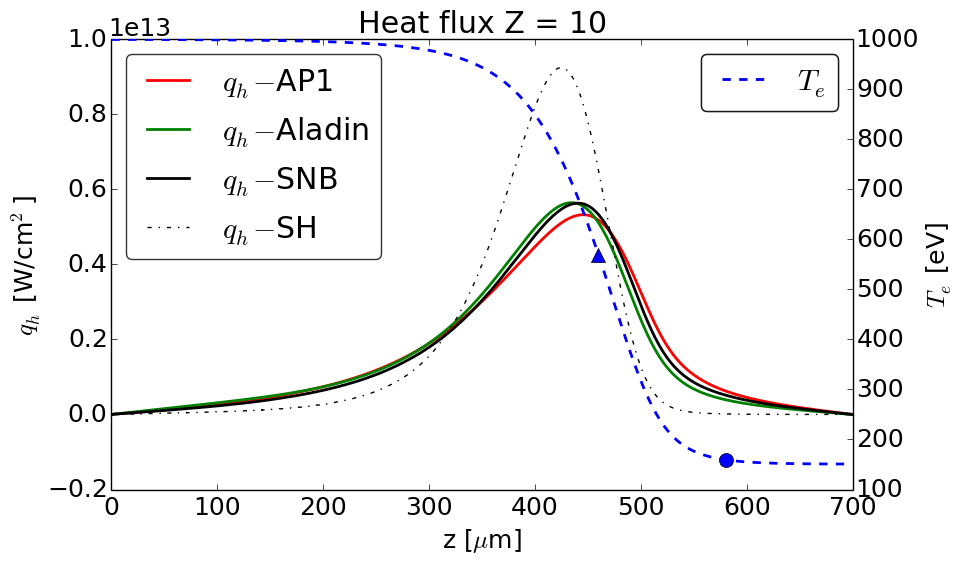
\includegraphics[width=\figscale\textwidth]{../VFPdata/C7_Aladin_case3_heatflux.png} \\
      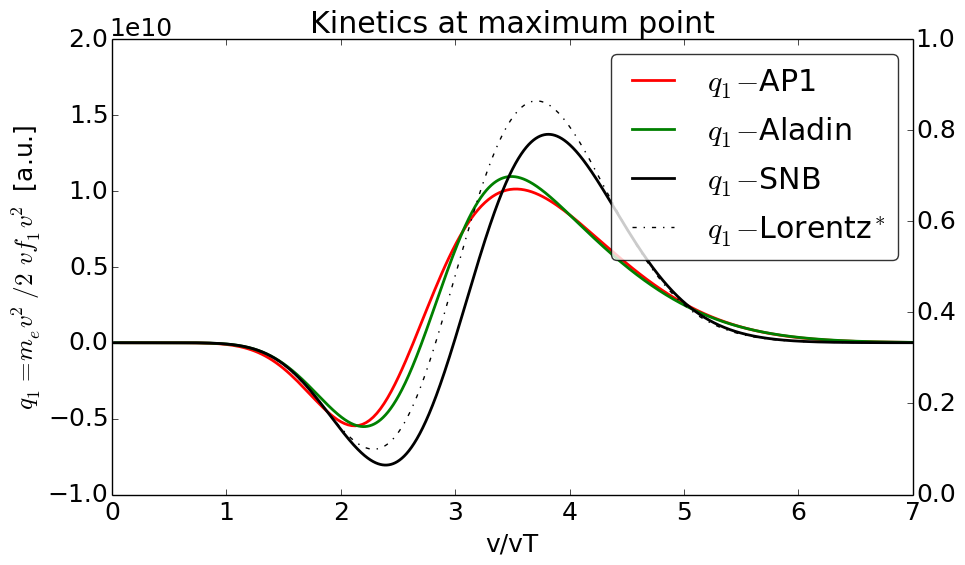
\includegraphics[width=\figscale\textwidth]{../VFPdata/C7_Aladin_case3_kinetics.png} \\
      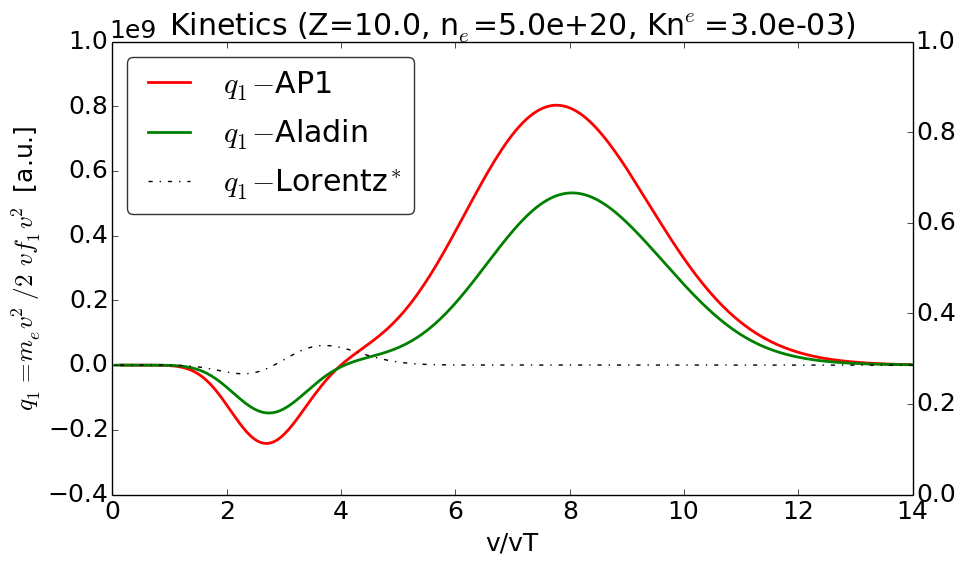
\includegraphics[width=\figscale\textwidth]{../VFPdata/C7_Aladin_case3_nonlocal_kinetics.png}  
    \end{tabular}
  \caption{  
  Snapshot 12 ps. Top: correct steady solution of heat flux.  
  Middle: correct comparison to kinetic profiles at point 460 $\mu$m by Aladin. 
  Velocity limit 3.3 $\vth$ at temperature 569.2 eV.
  Bottom: correct comparison to kinetic profiles at point 580 $\mu$m by Aladin.
  Velocity limit 13.1 $\vth$ at temperature 159.4 eV.
  }
  \label{fig:C7_Aladin_case3}
  \end{center} 
\end{figure}

\begin{figure}[tbh]
  \begin{center}
    \begin{tabular}{c}
      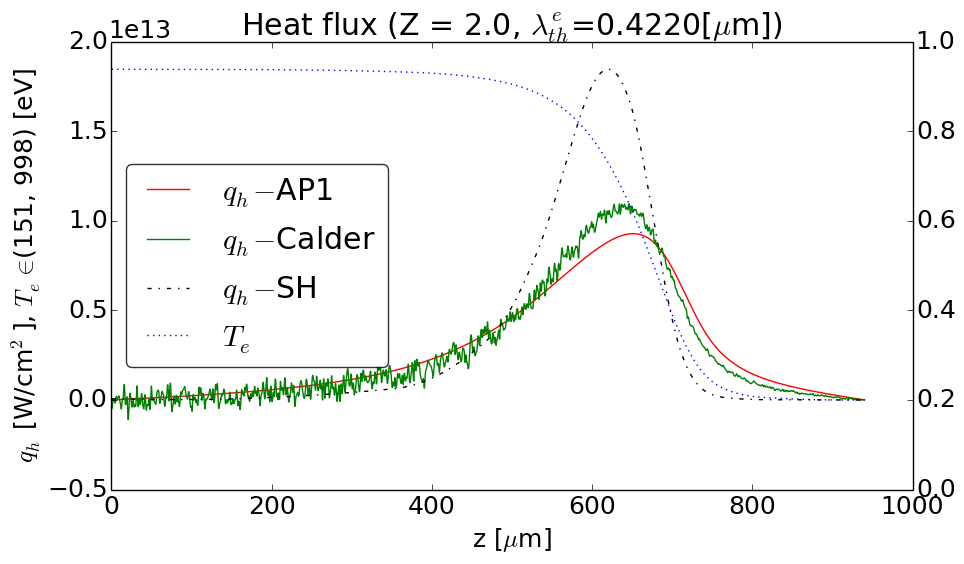
\includegraphics[width=\figscale\textwidth]{../VFPdata/C7_Calder_case1_heatflux.png} 
	  \\ 
	  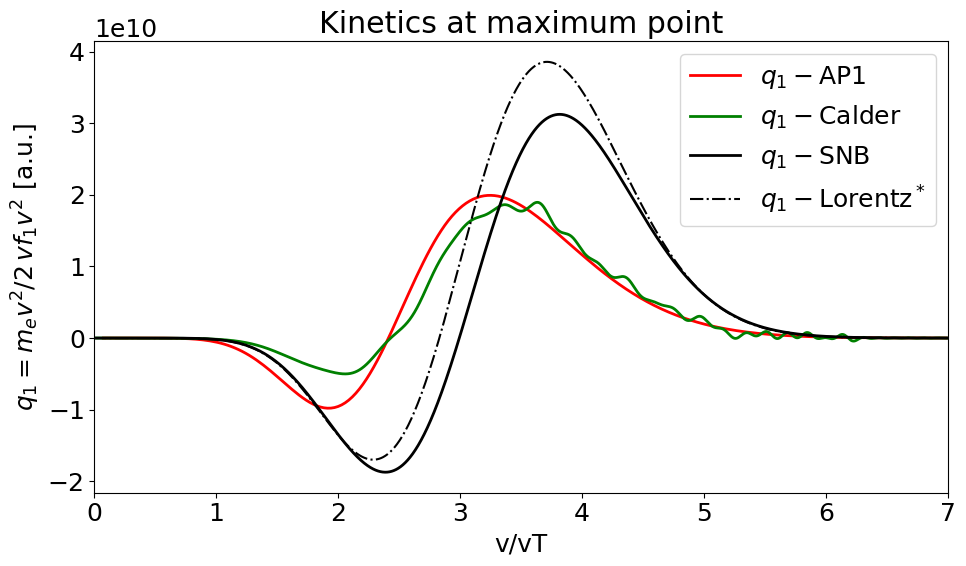
\includegraphics[width=\figscale\textwidth]{../VFPdata/C7_Calder_case1_kinetics.png}
	  \\ 
	  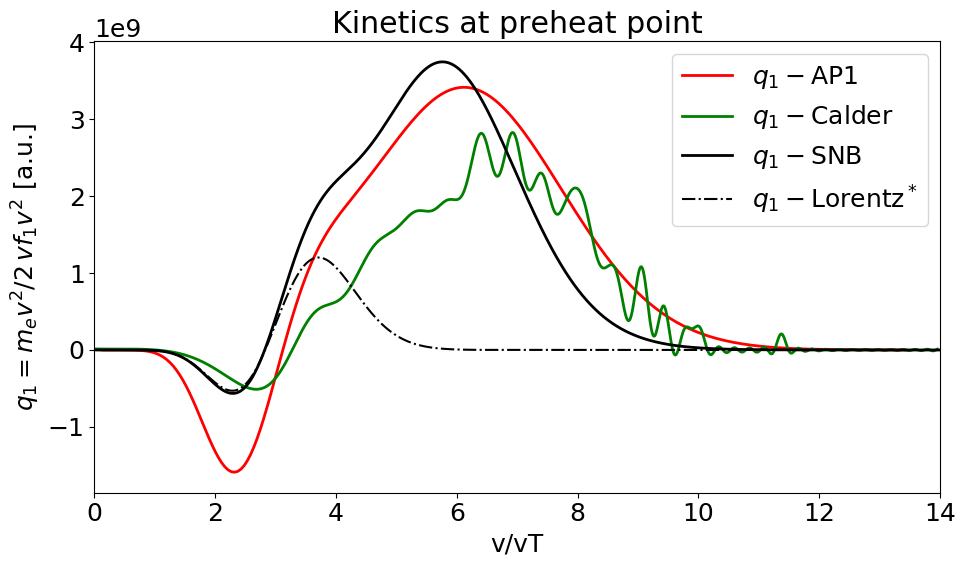
\includegraphics[width=\figscale\textwidth]{../VFPdata/C7_Calder_case1_nonlocal_kinetics.png}
    \end{tabular}
  \caption{  
  %Snapshot 11 ps. Left: correct steady solution of heat flux. 
  %Points 640 $\mu$m and 750 $\mu$m, corresponding velocity limit 3.8 $\vth$ 
  %and 7.4 $\vth$ on temperatures 662.3 eV and 198.0 eV.
  Snapshot 11 ps. Top: correct steady solution of heat flux.  
  Middle: correct comparison to kinetic profiles at point 640 $\mu$m by Calder. 
  Velocity limit 3.8 $\vth$ at temperature 662.3 eV.
  Bottom: correct comparison to kinetic profiles at point 750 $\mu$m by Calder.
  Velocity limit 7.4 $\vth$ at temperature 198.0 eV.
  }
  \label{fig:C7_Calder_case1}
  \end{center} 
\end{figure}

\subsection{Heat-bath problem}  
\label{sec:heatbath_test}

%\begin{figure}[tbh]
%  \begin{center}
%    \begin{tabular}{c}
%      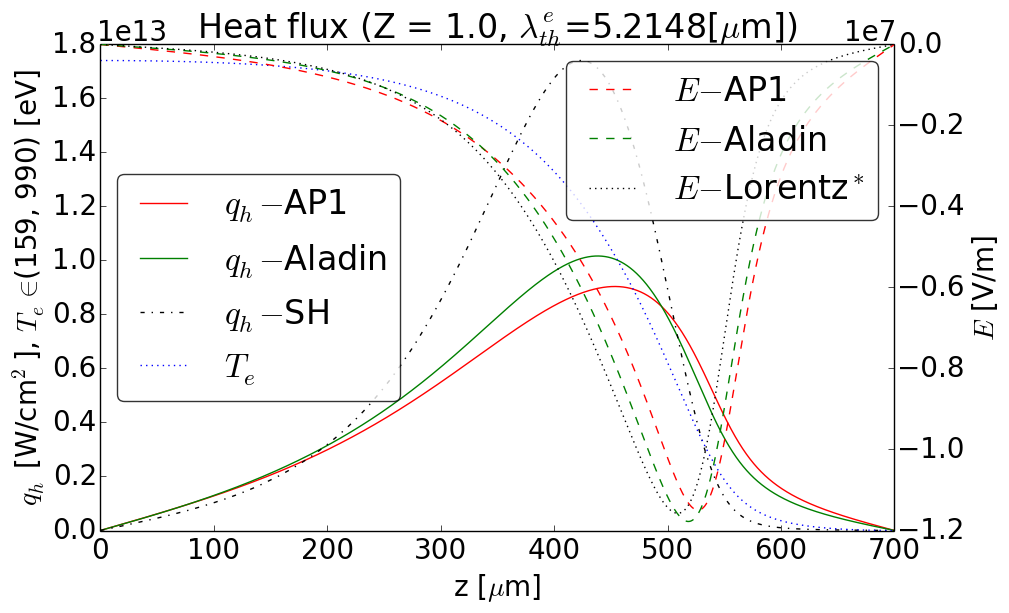
\includegraphics[width=\figscale\textwidth]{../VFPdata/C7_Aladin_case5_heatflux.png} \\
%      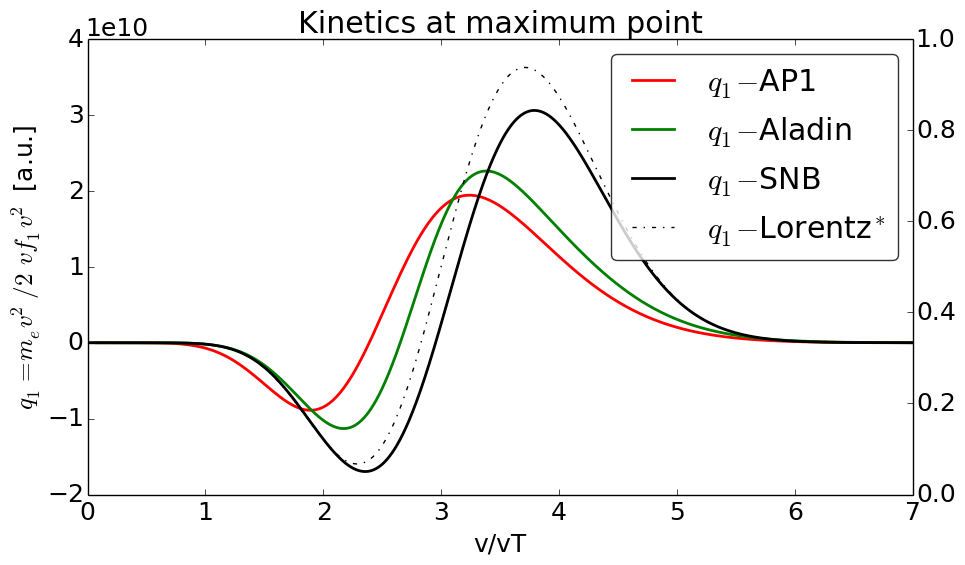
\includegraphics[width=\figscale\textwidth]{../VFPdata/C7_Aladin_case5_kinetics.png}
%    \end{tabular}
%  \caption{  
%  Snapshot 20 ps. Left: correct steady solution of heat flux. 
%  Right: Aladins results are correct. Velocity limit 4.4 $\vth$..
%  }
%  \label{fig:C7_Aladin_case5}
%  \end{center} 
%\end{figure}
\begin{figure}[tbh]
  \begin{center}
    \begin{tabular}{c}
      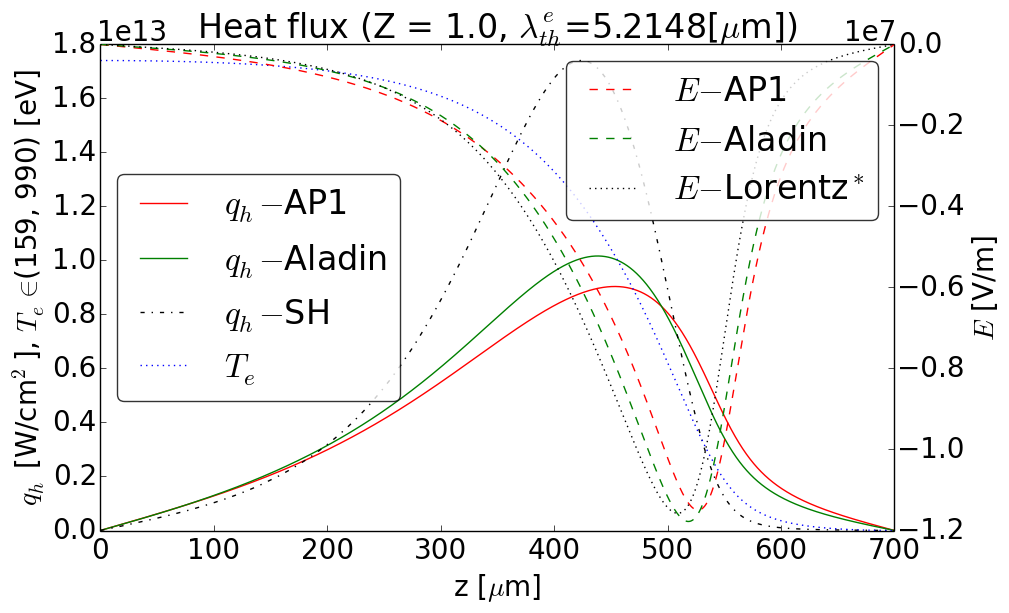
\includegraphics[width=\figscale\textwidth]{../VFPdata/C7_Aladin_case5_heatflux.png} \\
      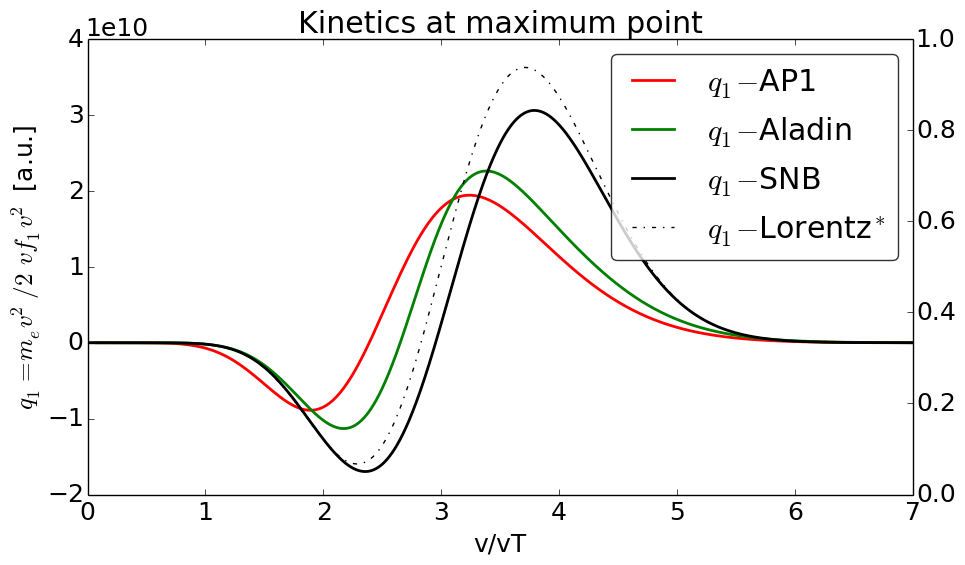
\includegraphics[width=\figscale\textwidth]{../VFPdata/C7_Aladin_case5_kinetics.png} \\
	  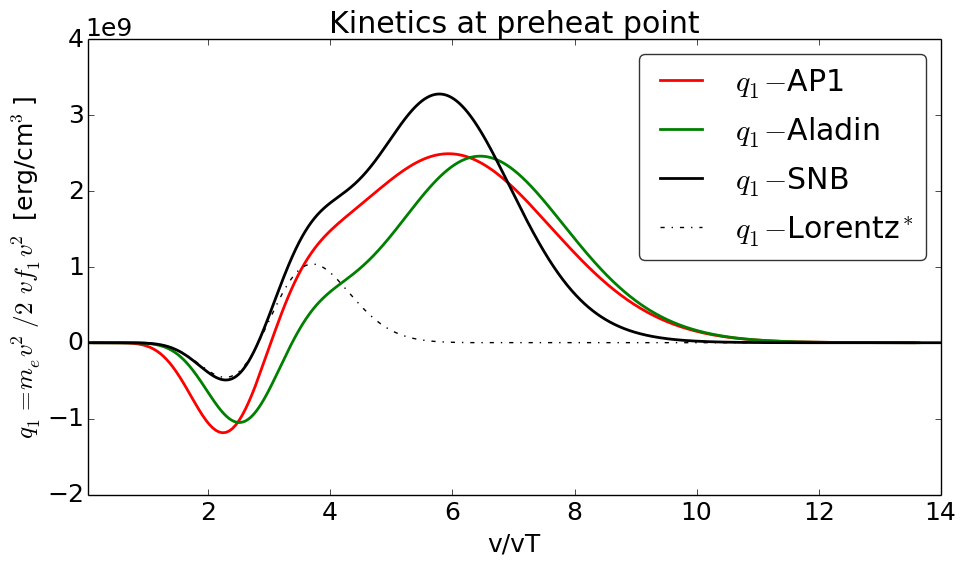
\includegraphics[width=\figscale\textwidth]{../VFPdata/C7_Aladin_case5_nonlocal_kinetics.png}
    \end{tabular}
  \caption{  
  Snapshot 20 ps. Top: correct steady solution of heat flux and electric field. 
  Middle: correct comparison to kinetic profiles at point 460 $\mu$m by Aladin. 
  Velocity limit 4.2 $\vth$ at temperature 622.4 eV.
  Bottom: correct comparison to kinetic profiles at point 580 $\mu$m by Aladin.
  Velocity limit 9.1 $\vth$ at temperature 192.3 eV.
  %Snapshot 20 ps. Top: correct steady solution of heat flux. 
  %Right: Aladins results are correct. Velocity limit 4.4 $\vth$.
  %Snapshot 20 ps. AP1 kinetic profiles at point 580~$\mu$m corresponding to 
  %a~highly nonlocal nature of the~heat flux %\figref{fig:C7_Aladin_case5} 
  %and is in a~good agreement with
  %\cite{Sherlock_PoP2017}. Velocity $max(q_1)$ = 6.0 $\vth$. 
  %Velocity limit 9.0 $\vth$.
  }
  \label{fig:C7_Aladin_case5}
  %\label{fig:C7_Aladin_case5_nonlocal}
  \end{center} 
\end{figure}

The accuracy of the AP1 is compared to Calder, Aladin, Impact, and SNB by 
calculating the heat flow in the case
where a~large relative temperature variation
\begin{equation}
  T_e(z) = 0.575 - 0.425 \tanh\left((z-450) s\right) ,
  \label{eq:T_init}
\end{equation}
which exhibits a~smooth steep gradient at point 450~$\mu$m 
connecting a~hot bath ($T_e = 1$~keV) 
and cold bath ($T_e = 0.17$~keV) and $s$ is the~parameter of steepness. 
This test is referred to as a~simple non-linear heat-bath problem and
originally was introduced in \cite{marocchino2013} and further investigated
in  \cite{Sorbo_2015, Sorbo_2016, Sherlock_PoP2017, Brodrick_PoP2017}.

%Aladin and Impact simulations showed an evolution of the heat flow
%from the local (due to initialising as a Maxwellian) to the
%nonlocal, with a reduced peak, over an initial transient
%phase (over which the temperature ramp flattened somewhat). 
%The transient phase was considered over when the
%ratio of the VFP heat flow to the expected local heat
%flow stopped decreasing. After the transient phase this
%ratio begins to slowly increase as the thermal conduction flattens 
%the temperature ramp and the ratio of the scalelength to mfp increases 
%(i.e. the thermal transport slowly becomes more local). 

The~total computational box size is 700 $\mu$m in the~case
of Aladin and Impact and 1000 $\mu$m in the~case of Calder.
We performed Aladin, Impact, and Calder simulations showing an~evolution of
temperature starting from the~initial profile \eqref{eq:T_init}. 
Due to the~initial distribution function being approximated by a~Maxwellian,
the~first phase of the~simulation exhibits a~transient behavior of the~heat
flux. After several ps the~distribution adjusts properly to its nonlocal nature
and the~heat flux profiles can be usefully compared. 
We then take the temperature profile from Aladin/Impact/Calder and used 
our AP1 and SNB implementations to calculate the heat flow
they would predict given this profile. 
For all heat-bath simulations the electron density, Coulomb logarithm and 
ionisation were kept constant and uniform.
The~coulomb logarithm was held fixed throughout, $\lnc = 7.09$.

We show AP1 results for various ionization states, namely $\Zbar= 10, 2, 1$ 
in \figref{fig:C7_Aladin_case3}, \figref{fig:C7_Calder_case1}, 
and \figref{fig:C7_Aladin_case5} respectively, corresponding to 
a~moderate nonlocality 
(Kn$^e \sim 10^{-2}$) leading to a~rouhgly 50 $\%$ inhibition compared 
to the~local SH heat flux maximum. 
It is preferable to use 
$\text{Kn}^e = \frac{\mfpe}{\sqrt{\Zbar + 1}L_{T_e}}$ instead of
 $\text{Kn} = \frac{\mfpei}{L_{T_e}}$, because $\sqrt{\Zbar + 1}$ provides 
a~better scaling of nonlocality with respect
to ionization \cite{LMV_1983_7}, i.e. the~flux inhibition and Kn$^e$ are
kept approximately the~same when varying $\Zbar$.
In addition to the~heat flux profiles, we also show the~distribution function 
details related to the~point of the~heat flux maximum (644 $\mu$m) 
and to the~point of the~nonlocal transport effect (750 $\mu$m) in the~form of
the~flux moment of EDFs anisotropic part \eqref{eq:q1}.
The~nonlocal transport effect shows a~very good agreement with 
previous results published in \cite{Sherlock_PoP2017}.

In the~top plot of \figref{fig:C7_Aladin_case3} we show heat flux profiles
computed by Aladin and AP1 corresponding to the~temperature $\Te$ profile 
computed by Aladin for $\Zbar = 10$. The~EDFs $q_1$ at the~crossed point of 
the~temperature profile is shown in the~middle plot, where a~very precise match
between AP1 and Aladin can be observed, and $q_1$ at the~circled point 
of the~temperature profile is shown in the~bottom plot. In the~latter case
AP1 shows a~very similar properties as Aladin with a~difference in magnitude
corresponding to a~higher heat flux computed by AP1 at this point.

In the~top plot of \figref{fig:C7_Calder_case1} heat flux profiles
computed by Calder and AP1 corresponding to the~temperature $\Te$ profile 
computed by Calder are shown for $\Zbar = 2$. 
Very good match of $q_1$ can be seen between 
AP1 and Calder at the~crossed point of the~temperature profile in the~middle 
plot and $q_1$ at the~circled point of the~temperature profile is shown 
in the~bottom plot. In the~latter case AP1 shows a~very similar properties 
as Calder with a~difference in magnitude corresponding to a~higher heat flux 
computed by AP1 at this point. In general, Calder exhibits a~lack of 
return current (negative part of $q_1$), i.e. the~electron number is not 
exactly conserved. This probably arises from the~nature of the~Monte Carlo 
method used to solve \eqref{eq:LBB_model} and its sensitivity to Gauss law
of charge conservation.

Similar to \figref{fig:C7_Aladin_case3}, but for $\Zbar = 1$, 
the~heat flux profiles, $q_1$ at the~heat flux maximum (crossed point) and
at~the~nonlocal transport region (circled point) computed by Aladin and AP1 
are shown in \figref{fig:C7_Aladin_case5}. It should be noted, 
that the~difference in $q_1$ resembles to the~low $\Zbar$ trend
shown in \figref{fig:q1s_summary} and that AP1 compares very well
to Aladin. We also add the~electric field profiles
in the~top plot of \figref{fig:C7_Aladin_case5}. 
One can see that $\E$ does not change much in magnitude, but
it is displaced in direction down the~temperature gradient thus causing 
a~significant modification compared to the~local $\E_L$ values.
In general, a~very good performance of AP1 model equations 
\eqref{eq:AP1f0}, \eqref{eq:AP1f1}, and \eqref{eq:AmpereKinetic} 
(no B field in 1D) can be observed in all three cases when compared
to the~computed results by Aladin and Calder.

In addition, the~Knudsen number Kn$^e$ has been varied among the~simulation 
runs in order to address a~broad range of nonlocality of 
the~electron transport corresponding 
to the~laser-heated plasma conditions, i.e. Kn$^e \in (0.0001, 1)$. 
The~variation of Kn$^e$ arises from the~variation
of the~uniform electron density $n_e \in (10^{19}, 10^{23})$ cm$^{-3}$ or 
the~length scale given by the~slope of the~temperature profile 
$s \in (1/2500, 1/25) \mu$m. Results of an~extensive set of simulations of
varying Kn$^e$ is shown in \figref{fig:Kn_results}.
 
\begin{figure}[tbh]
  \begin{center}
    \begin{tabular}{c}
      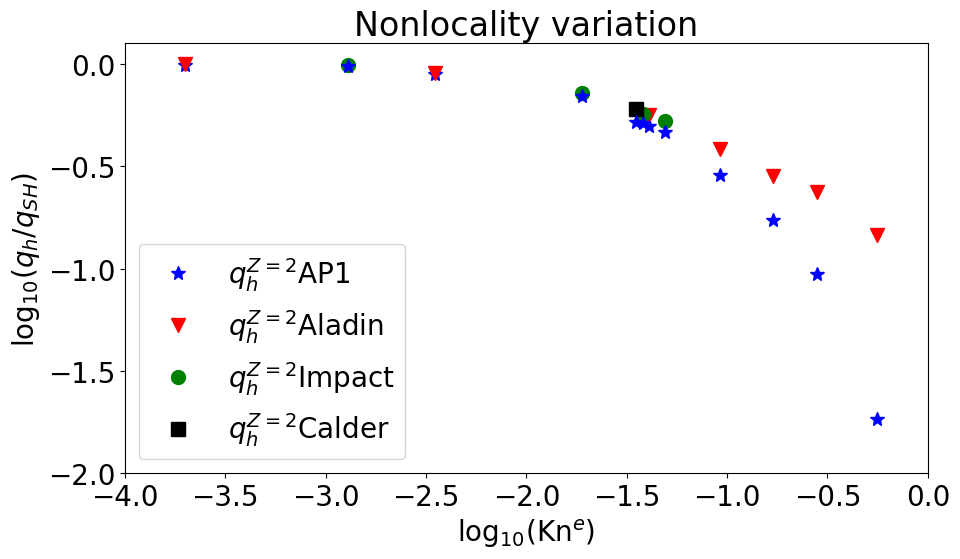
\includegraphics[width=\figscale\textwidth]{Kn_results.png}
    \end{tabular}
  \caption{  
  Simulation results for the case $Z=2$ computed by AP1/Aladin/Impact/Calder.
  Every point corresponds to the maximum heat flux in a "tanh" temperature 
  simulation, which can be characterized by Kn. The range of 
  $\log_{10}(\text{Kn})\in (0, -4)$ can be expressed as equivalent 
  to the~electron density approximate range n$_e \in (1e19, 3.5e22)$ of 
  the~50 $\mu$m slope tanh case. In the case of Kn = 0.56, 
  $q_{Aladin} / q_{AP1}\approx 7.9$.}
  \label{fig:Kn_results}
  \end{center} 
\end{figure}
When analyzing the~results of \figref{fig:Kn_results} we have found 
an~important observation related to the~stopping effect of electrons.
It turns out, that the~force acting on electrons is dominated by directional
electric field above some velocity limit $\vmag_{lim}$ and this limit drops 
down significantly when the~plasma conditions are more nonlocal, 
i.e. with increasing Knudsen number as can be seen in \tabref{tab:vlim}. 
As a~consequence, one can see
that when Kn$^{e} \sim 10^{-1}$ the~electrons responsible for the~heat flux
(velocity $\sim$ 3.5 $\vth$) are preferably affected by the~electric field
rather than by collisions.

\begin{table}
\begin{center}
  \begin{tabular}{c|ccccc}
    \hline\hline\\
    %Kn$^e$ & $10^{-4}$ & $10^{-3}$ & $10^{-2}$ & $10^{-1}$ & $1$ \\\\
    Kn$^e$ & $\,\,10^{-4}\,\,$ & $\,\,10^{-3}\,\,$ & $\,\,10^{-2}\,\,$ & $\,\,10^{-1}\,\,$ & $\,\,1\,\,$ \\\\
    \hline\\
    $\vmag_{lim} / \vth$ & 70.8 & 22.4 & 7.3 & 3.1 & 1.8\\\\
    \hline\hline
  \end{tabular}
  \caption{
  Scan over varying nonlocality (Kn$^e$) showing the~limit of 
  the~collision friction dominance over the~acceleration of electrons 
  due to the~electric field force. The~electric field effect is dominant
  for electrons with higher velocity than $\vmag_{lim}$ defined in 
  \eqref{eq:v_limit}. Kn$^e$ and $\vth$ are evaluated from the~same 
  plasma profiles.
  %$\sqrt{3}\vmag\frac{\me}{2\qe}\nue > |\E|$.
  }
\label{tab:vlim}
\end{center}
\end{table}

Yet another observation can be made when analysing $q_1$ 
in \figref{fig:C7_Aladin_case3}, \figref{fig:C7_Calder_case1}, and 
\figref{fig:C7_Aladin_case5}. When comparing their middle and bottom plots,
both velocity maxima of the~EDF correspond to approximately same velocity
for each of the~cases, i.e. that the~electrons responsible for the~flux in
the~bottom plot are those flux dominating electrons from the~heat flux
maximum point shown in the~middle plot. Notice that different reference 
temperatures and $\vth$ are used in the~middle and bottom plots. 
This provides a~microscopic information
about the~motion of electrons on the~nonlocal spatial scale. 

In every simulation run of AP1 we used 250~velocity groups in order to avoid
numerical errors in modeling of the~electron kinetics. However, a~smaller 
number of groups, e.g. 50, provides a~very similar results 
(an~error around 10$\%$ in the~heat flux). 
\textit{Here gather and provide a brief summary about the simulation input of
Aladin, Impact, and Calder.}

\subsection{Hohlraum problem}
Additionally to the~steep temperature gradients, the~laser-heated plasma 
experiments also involve steep density gradients and variation in ionization,
which is even more dominant in multi-material targets as in inertial
fusion experiments, e.g. at the interface between the helium gas-fill and 
the ablated high $\Zbar$ plasma.

In~\cite{Brodrick_PoP2017}, a~kinetic simulation of such a~test was introduced.
Plasma profiles provided by a~HYDRA simulation in 1D spherical
geometry of a~laser-heated gadolinium hohlraum containing a~typical helium 
gas-fill were used as input for the~IMPACT \cite{Kingham_JCP2004} VFP code.  
For simplicity, the Coulomb logarithm was treated as a
constant $\lnc_{ei}$ = $\lnc_{ee}$ = 2.1484. In reality, in the~low-density 
corona $\lnc$ reaches 8, which, however, does not affect the~heat flux profile 
significantly. Plasma profiles at 20 nanoseconds of the~HYDRA simulation 
were used (after spline smoothing) as the~initial conditions for 
the~IMPACT run (in planar geometry).

\figref{fig:Gd_VFP_10ps_heatflux} shows the~electron temperature $\Te$ 
evolved during 10 ps by Impact, and the~electron density $\ed$ and 
ionization $\Zbar$ profiles. Along with plasma profiles the~heat flux profiles
of AP1, Impact, and SNB are also shown. 
\textit{Kn profile will be probably added}. One can observe an~overall good
match among models in the~preheat region.

\begin{figure}[tbh]
  \begin{center}
    \begin{tabular}{c}
      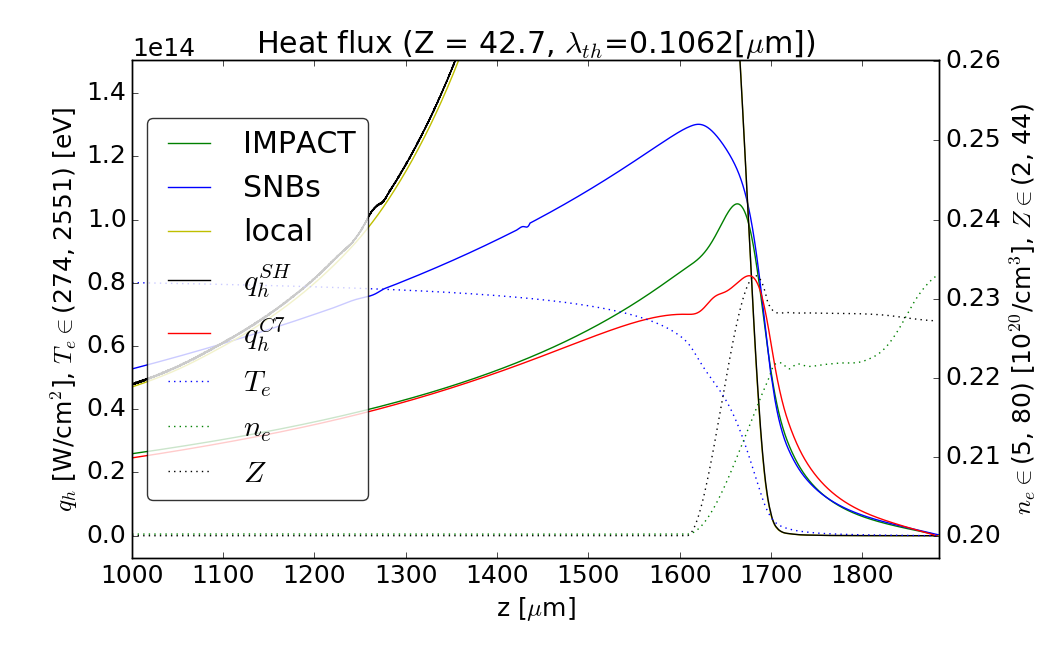
\includegraphics[width=\figscale\textwidth]{../VFPdata/GD_Hohlraum/fluxes_10ps.png} 
    \end{tabular}
  \caption{
  Heat flux profiles by AP1, Impact and SNB along 
  the~electron temperature $\Te$, electron density $\ed$, 
  and ionization $\Zbar$ profiles in a~laser-heated gadolinium hohlraum 
  containing a helium gas-fill.
  }
  \label{fig:Gd_VFP_10ps_heatflux}
  \end{center} 
\end{figure}

It is worth mentioning that in the~surroundings of the~heat flux maximum 
($\sim 1662 \mu$m) the~profiles of all plasma variables exhibit steep gradients 
with a change from $T_e$ = 2.5 keV, $n_e$ = 5$\times$10$^{20}$ cm$^{−3}$, 
$\Zbar$ = 2 to $T_e$ = 0.3 keV, $n_e$ = 6$\times$10$^{21}$ cm$^{−3}$ , 
$\Zbar$ = 44 across approximately 100 $\mu$m 
(between 1600~$\mu$m and 1700~$\mu$m), starting at the~helium-gadolinium 
interface.  
In this region, we can see a~qualitative match between AP1 and Impact, however,
we observe that the~electric field limit \appref{app:AP1limit} leads to 
the~drop of the~AP1 heat flux on the~material interface, which then aligns to 
the~Impact heat flux in the~corona appropriately. On the~other hand, 
SNB exhibits a~significant heat flux overestimation in both
the~steep gradients region and in the~plasma corona. We also attribute this
to the~lack of proper action of the~electric field (the~directional effect) 
in the~SNB approach.

%
